	\documentclass[12pt]{article}

%% Language and font encodings
\usepackage[english]{babel}
\usepackage[utf8x]{inputenc}
\usepackage[T1]{fontenc}

%% Sets page size and margins
\usepackage[a4paper,top=2cm,bottom=2cm,left=2cm,right=2.5cm,marginparwidth=1.75cm]{geometry}

%% Useful packages
\usepackage{amsmath}
\usepackage{amsfonts}
\usepackage{graphicx}
\usepackage[colorinlistoftodos]{todonotes}
\usepackage[colorlinks=true, allcolors=blue]{hyperref}

\title{Homework 7}
\author{Motoaki Takahashi}
\date{}

\begin{document}
\maketitle
\section*{Question 1}
I followed the iteration method suggested by p.3 in the question sheet. The iteration converges only when I set the dampning parameter $\lambda = 0.1\, \text{or}\, 0.2$.\par
Figure 1 shows firm 1's values against firm 1 and firm 2's states. The vertical axis shows the values and the horizontal axis to the left (resp. right) shows firm 1 (resp. 2)'s states. 
\begin{figure}[h]
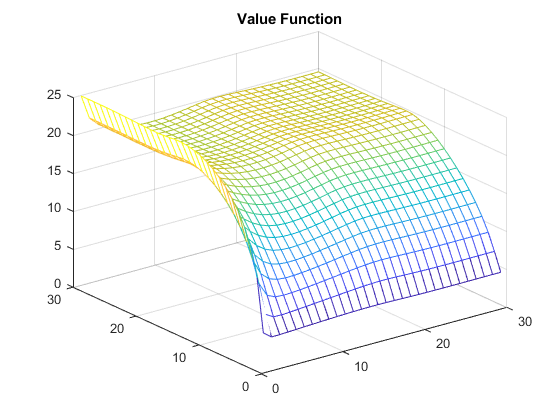
\includegraphics[width=\textwidth]{1.png}
\caption{Value function}
\end{figure}
\clearpage
Figure 2 shows the policy function of firm 1. The vertical axis shows the price set by firm 1 and the horizontal axes are the same as in Figure 1.
\begin{figure}[h]
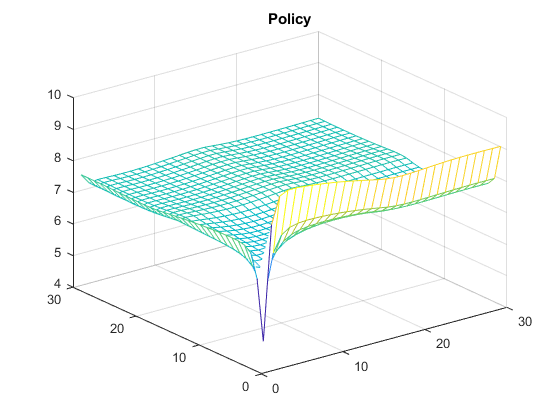
\includegraphics[width=\textwidth]{2.png}
\caption{Policy function}
\end{figure}
\clearpage
\section*{Question 2}
I made a $900\times900$ matrix that represents the transition matrix from $(\omega_1, \omega_2)$ to the next period's $(\omega_{1}', \omega_{2}')$.\par
Figure 3 plots the distribution of states after 10 periods. The vertical axis shows the likelihood of the states.
\begin{figure}[h]
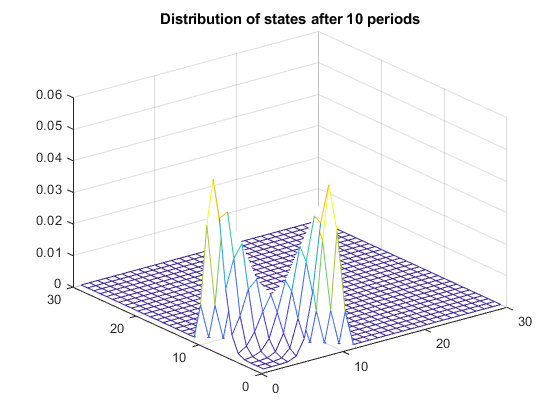
\includegraphics[width=\textwidth]{3.png}
\caption{States after 10 periods}
\end{figure}
\clearpage
Figure 4 plots the distribution of states after 20 periods.
\begin{figure}[h]
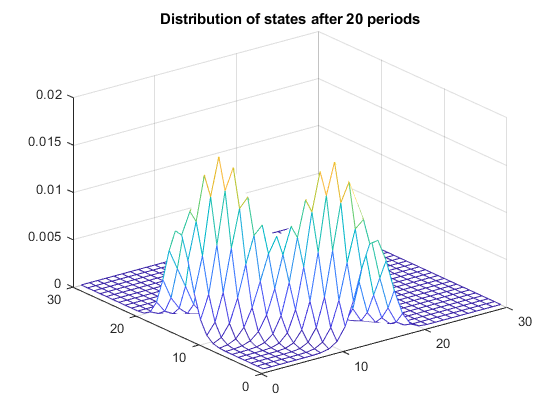
\includegraphics[width=\textwidth]{4.png}
\caption{States after 20 periods}
\end{figure}
\clearpage
Figure 5 plots the distribution of states after 30 periods.
\begin{figure}[h]
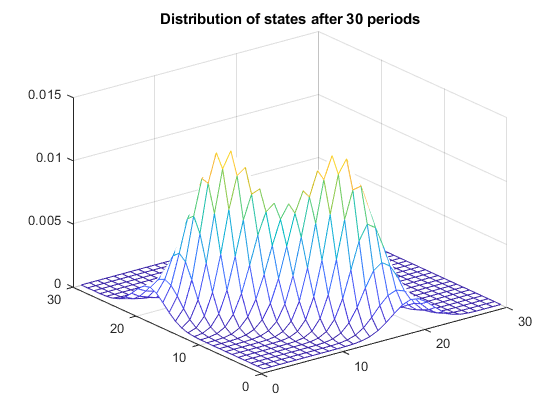
\includegraphics[width=\textwidth]{5.png}
\caption{States after 30 periods}
\end{figure}
\clearpage
\section*{Question 3}
I multiply the transition matrix to an arbitrary initial state vector repeatedly, until the distribution of the states converges.\par
Figure 6 plots the stationary distribution of the states.
\begin{figure}[h]
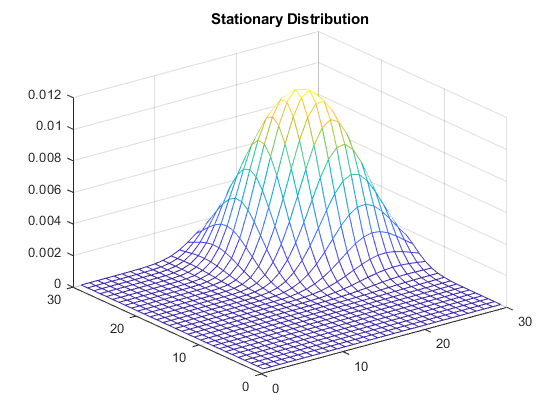
\includegraphics[width=\textwidth]{6.png}
\caption{Stationary Distribution}
\end{figure}

\end{document}